\documentclass[aspectratio=169,11pt]{beamer}
% Shared preamble for the CogLean decks.
% Build the slides alone, or with speaker notes (see the Makefile):
%   pdflatex deck.tex                                   -> slides
%   pdflatex -jobname=deck-notes "\def\withnotes{}\input{deck.tex}"  -> slides + notes
\usetheme{default}
\usecolortheme{seahorse}
\setbeamertemplate{navigation symbols}{}
\setbeamertemplate{footline}[frame number]
\setbeamerfont{note page}{size=\small}
\ifdefined\withnotes
  \setbeameroption{show notes}
\fi
\usepackage[T1]{fontenc}
\usepackage{lmodern}
\usepackage{booktabs}
\usepackage{amsmath,amssymb}
\usepackage{tikz}
\usetikzlibrary{positioning,arrows.meta,shapes.misc}
\tikzset{
  box/.style={draw, rounded corners, align=center, minimum height=8mm, inner sep=4pt, fill=blue!6},
  arr/.style={-{Stealth[length=2mm]}, thick}
}
\newcommand{\code}[1]{\texttt{#1}}
\newcommand{\has}{\textbf{has}}
\newcommand{\lacks}{\textcolor{red!70!black}{lacks}}
\newcommand{\never}{\textcolor{red!70!black}{\textbf{never}}}
\newcommand{\canhold}{can hold}


\title{CogLean}
\subtitle{A machine-checked library of cognitive theory}
\author{Jeff Shrager}
\date{October 2026}

\begin{document}

\begin{frame}
  \titlepage
\end{frame}
\note{
\begin{itemize}
\item This talk is about a way of stating cognitive theories so that what follows from them can be checked, compared, and accumulated.
\item The vehicle is Lean, a programming language that is also a proof checker. You don't need to know Lean to follow this talk.
\item The library is open source: github.com/jeffshrager/CogLean.
\end{itemize}
}

\begin{frame}{The problem}
  Cognitive theories are stated in prose, in simulation code, or as equations fitted to data.
  \bigskip
  \begin{itemize}
    \item What follows from a theory's \emph{core assumptions}, as distinct from its parameter settings or implementation details, is rarely checked.
    \item A simulation shows that a model \emph{can} produce a result, with these parameters and these stimuli.
    \item It doesn't show which assumptions produced it, whether it survives other parameters, or whether a rival theory would produce it just as well.
  \end{itemize}
\end{frame}
\note{
\begin{itemize}
\item Most modelling evidence is a fit: one model, one set of parameters, compared with data.
\item That's valuable, but it leaves three questions open: which assumptions did the work, is the result robust, and does it discriminate between theories?
\item The rest of the talk is about answering those questions with proofs.
\end{itemize}
}

\begin{frame}{Three kinds of evidence a theory can give}
  \small
  \begin{tabular}{p{0.3\linewidth}p{0.3\linewidth}p{0.3\linewidth}}
    \toprule
    \textbf{One run} & \textbf{Every run} & \textbf{Every model satisfying the postulates}\\
    \midrule
    one model, one parameter setting & one model, all its executions & all models the theory allows\\
    the theory \emph{can} do it & that model \emph{always} does it & the postulates \emph{entail} it\\
    simulation & model checking, sweeps & proof\\
    \bottomrule
  \end{tabular}
  \bigskip

  CogLean is built around the third kind, and keeps the other two in the same language.
\end{frame}
\note{
\begin{itemize}
\item A theorem quantified over every model satisfying the postulates says which assumptions matter (the proof uses some and not others), what is robust, and whether a claim is possibility or necessity.
\item Simulation is still essential: it explores, suggests conjectures, and fits data. Proof settles which conjectures follow from which assumptions. Experiments with people decide whether the assumptions are right.
\end{itemize}
}

\begin{frame}{Why Lean}
  \begin{itemize}
    \item \textbf{One definition, run and proved.} The same definition of a memory can be \emph{run} on an experiment's stimuli and \emph{proved about} for all stimuli. The simulation and the theory can't drift apart.
    \item \textbf{Checked.} Every proof step is checked by a small trusted kernel.
    \item \textbf{General.} A theorem can quantify over all nets, all parameter values, all stimulus lists.
    \item \textbf{Cumulative.} Like Mathlib for mathematics: definitions made once, theorems imported rather than re-derived.
  \end{itemize}
  \bigskip
  \textit{The guarantee is relative.} Lean checks that a theorem follows from the definitions, not that the definitions capture the theory, still less that the theory is true of people.
\end{frame}
\note{
\begin{itemize}
\item Mathlib is a single, shared, machine-checked library of mathematics. CogLean aims at the same thing for cognitive theory.
\item The caveat on this slide matters and will come back: proofs are only as faithful as the formal definitions.
\end{itemize}
}

\begin{frame}{What is in the library}
  \begin{itemize}
    \item \textbf{CogLib}: shared constructs (feature codes, exact probability distributions, discrimination nets, sampled retrieval, attention) and theory-neutral phenomena.
    \item \textbf{EPAM} (Feigenbaum): discrimination-net learning. Stimulus generalization, oscillation, retroactive inhibition, learning to criterion, the serial position effect: all proved. A published serial-anticipation run is reproduced (33--34 of 34 responses agree).
    \item \textbf{Strategy choice} (Siegler \& Shrager): distributions of associations. Retrieval is used with probability $1-(1-R)^n$; and a finding: a more peaked distribution can \emph{raise} overt strategy use.
    \item \textbf{Multi-digit addition}: the two combined, with 18 predictions neither makes alone.
  \end{itemize}
\end{frame}
\note{
\begin{itemize}
\item Every theorem is fully proved, with no gaps, and uses only Lean's standard axioms.
\item The peakedness result is a good example of what proof buys: an intuitive claim from the original chapter needs a condition the chapter doesn't state.
\end{itemize}
}

\begin{frame}{The generality problem}
  There are a great many specific models: EPAM, ACT-R, SAM, REM, MINERVA~2, TODAM, connectionist networks\ldots
  \bigskip
  \begin{itemize}
    \item Formalizing them one at a time doesn't scale.
    \item A pile of formalized models doesn't say what any two of them \emph{disagree} about.
    \item And none of them is ``true'': unlike mathematics, there's no settled foundation to build on.
  \end{itemize}
\end{frame}
\note{
\begin{itemize}
\item This is the central design question. The answer on the next slides is to organize the library around laws, the way Mathlib organizes algebra.
\end{itemize}
}

\begin{frame}{Laws and families}
  \begin{columns}[T]
    \column{0.5\textwidth}
    \textbf{Laws}: small, theory-neutral properties of a memory.
    \begin{itemize}\small
      \item \emph{Certainty}: a just-studied item is retrieved for certain.
      \item \emph{Stability}: studying one item doesn't change another's retrieval.
      \item \emph{Order-freedom}: the order of study doesn't matter.
      \item \emph{Recency}: the later of two similar items is favoured.
      \item \emph{Stored-only}: nothing unstudied is retrieved.
      \item \emph{Determinacy}: retrieval has a single outcome.
    \end{itemize}
    \column{0.5\textwidth}
    \textbf{Families}: mechanisms, each formalized once with its parameters free.
    \begin{itemize}\small
      \item Discrimination (EPAM)
      \item Activation (ACT-R declarative memory)
      \item Strength with a criterion (DOA)
      \item Global matching (MINERVA~2)
    \end{itemize}
    \bigskip
    Predictions are proved \emph{from laws}, not from models.
  \end{columns}
\end{frame}
\note{
\begin{itemize}
\item Mathlib doesn't formalize every group; it proves theorems once per law (monoid, group, ring), and particular structures inherit them.
\item Here, a prediction reads ``any memory with stability predicts no interference with practiced items'', not ``EPAM predicts\ldots''.
\end{itemize}
}

\begin{frame}{The theory matrix}
  \small
  \begin{tabular}{lcccccc}
    \toprule
    & Certainty & Stability & Order-free & Recency & Stored-only & Determinate\\
    \midrule
    Discrimination & \has & \has & \lacks & \lacks & \has & \has\\
    Activation & \lacks & \lacks & \lacks & \has & \has & \lacks\\
    Strength & \lacks & \lacks & \has & \lacks & \has & \lacks\\
    Global matching & \lacks & \lacks & \has & \lacks & \lacks & \has\\
    \bottomrule
  \end{tabular}
  \bigskip

  Every cell is a theorem: a general proof (\has), or a counterexample (\lacks).
  Every law separates some families, and every family has its own row.
\end{frame}
\note{
\begin{itemize}
\item ``Has'' cells hold for every parameter choice meeting stated conditions. ``Lacks'' cells are single counterexamples on small stimulus sets; where in its parameter space a family does have a law is further work.
\item Global matching was added as a test. On the first four laws it looked exactly like strength memory, which forced the stored-only law: global matching's output is a blend, which can be a prototype never studied.
\item The activation family here is ACT-R with decay 1 and temperature 1, where all its quantities are rational and exactly computable.
\end{itemize}
}

\begin{frame}{What is true here?}
  In mathematics, a proved theorem is true. Here there are only competing theories. What can a library build on?
  \bigskip
  \small
  \begin{tabular}{p{0.32\linewidth}p{0.36\linewidth}p{0.22\linewidth}}
    \toprule
    Claim & Example & Status\\
    \midrule
    A law entails a prediction & stability $\Rightarrow$ practiced items stay practiced & proved, permanent\\
    A family has a law & discrimination nets have stability & proved, permanent\\
    People have a law & people lack stability in recall & empirical, revisable\\
    \bottomrule
  \end{tabular}
  \bigskip

  \normalsize
  Which theory is right follows from the second and third rows together.
\end{frame}
\note{
\begin{itemize}
\item The conditional results don't expire. They stay true even if every family in the library is refuted.
\item Mathlib is in the same position more often than it seems: it proves facts about Euclidean and non-Euclidean geometry alike, and leaves to physics which one space is.
\end{itemize}
}

\begin{frame}{A refutation spreads}
  \begin{itemize}
    \item If people lack a law, every family that has it is refuted at once, and every prediction proved from it loses its support, in every theory that uses it.
    \item The matrix carries a judged evidence row, kept apart from the theorems.
    \item Each judgment states its \textbf{bridge}: the assumption connecting what experiments measure (reports, decisions) to what a law is about (what memory retrieves).
  \end{itemize}
  \bigskip
  \textit{Example.} People endorse a prototype they never saw. That does not show they \emph{retrieved} it: a memory that returns a similar studied item also calls the prototype ``old''. The bridge is the missing piece.
\end{frame}
\note{
\begin{itemize}
\item As judged now: people lack certainty and order-freedom, have recency; stability and stored-only are mixed. Activation fits every settled entry; but each fit is a hypothesis, because the bridges are unformalized.
\item The lesson: the next step for theory comparison is often not more data but an explicit response model.
\end{itemize}
}

\begin{frame}{Example 1: confident errors, inherited}
  \begin{center}
  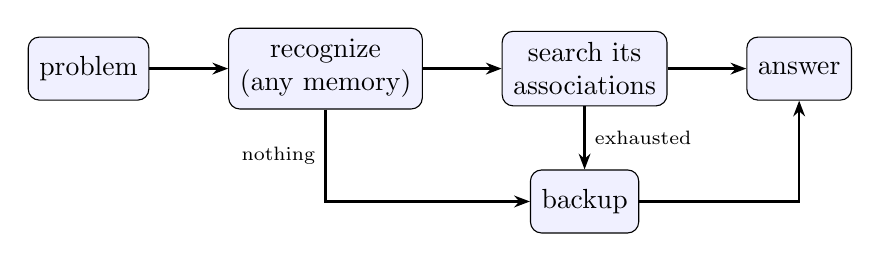
\begin{tikzpicture}[node distance=10mm]
    \node[box] (p) {problem};
    \node[box, right=of p] (r) {recognize\\(any memory)};
    \node[box, right=of r] (s) {search its\\associations};
    \node[box, below=8mm of s] (b) {backup};
    \node[box, right=of s] (a) {answer};
    \draw[arr] (p) -- (r); \draw[arr] (r) -- (s); \draw[arr] (s) -- (a);
    \draw[arr] (r) |- node[pos=0.25, left]{\scriptsize nothing} (b);
    \draw[arr] (s) -- node[right]{\scriptsize exhausted} (b);
    \draw[arr] (b) -| (a);
  \end{tikzpicture}
  \end{center}
  \begin{itemize}\small
    \item \textbf{Theorem}: a stranger taken for a familiar item with sharp associations is answered wrongly every time an answer is retrieved, with no more backup use than the familiar item.
    \item Proved once, for the composition. Inherited by multi-digit addition ($150+100$ taken for $100+100$) and by face naming (a stranger misnamed).
    \item From laws: any memory with determinacy, certainty and stability gives it. In the matrix, only discrimination.
  \end{itemize}
\end{frame}
\note{
\begin{itemize}
\item The distributions-of-associations model alone can't produce these errors: there, errors and backup use come from the same distribution and rise together. Confusion gives a problem another problem's distribution.
\item With ACT-R's memory, the errors are graded instead, and strangers say ``don't know'' more often.
\item The evidence judges that people lack certainty, so a graded version of the theorem is what would explain confident errors in people.
\end{itemize}
}

\begin{frame}{Example 2: an experiment derived from laws}
  Recency and order-freedom disagree. Derive the experiment that separates them.
  \medskip
  \begin{itemize}\small
    \item Two new items A and B; a probe equally similar to both.
    \item Study A then B, or B then A; then probe. Order effect $\Delta$ = how much more B is favoured after AB than after BA.
    \item \textbf{From laws alone}: order-freedom gives $\Delta = 0$; recency gives $\Delta > 0$; no memory has both.
    \item With a forced-choice response model, the prediction survives only if guessing is unbiased (or ``neither'' is equally likely in both orders).
  \end{itemize}
  \medskip
  \small
  \begin{tabular}{lccc}
    \toprule
    & ACT-R & Strength, MINERVA & EPAM\\
    \midrule
    $\Delta$ & $10/17$ (recency) & $0$ & $0$, or $-2$ (primacy)\\
    \bottomrule
  \end{tabular}
\end{frame}
\note{
\begin{itemize}
\item This reverses the usual workflow: start from a formal disagreement, derive the experiment, prove the separation.
\item EPAM has neither law. Its order effect comes from the shape of the net, not from time: after a suitable prior item, whichever of A and B is learned first always wins.
\end{itemize}
}

\begin{frame}{A related approach: SFT-GMA}
  \small
  Fisher, Houpt, Larue \& Schmidt (2024): critical tests of ACT-R from its core assumptions, by systems factorial technology (SFT) with global model analysis.
  \medskip
  \begin{columns}[T]
    \column{0.42\textwidth}
    \textbf{Shared}
    \begin{itemize}\footnotesize
      \item Separate a theory's \emph{core} assumptions from auxiliary choices.
      \item Derive critical tests from what the core forbids.
      \item Theorem-based: qualitative classes of models, not fits.
    \end{itemize}
    \column{0.56\textwidth}
    \textbf{Different} (as far as the abstract shows)
    \begin{itemize}\footnotesize
      \item \textbf{Constrains}: processing structure in response times (serial or parallel, stopping rule, dependence, capacity), not what memory retrieves.
      \item \textbf{Space}: SFT's established classes, with a paradigm and diagnostics linking them to data; CogLean's laws are new, and their link to data isn't formal yet.
      \item \textbf{Scope}: one architecture, not a matrix of families.
      \item \textbf{Checking}: CogLean's proofs are machine-checked; the abstract doesn't say how SFT-GMA's are derived.
    \end{itemize}
  \end{columns}
\end{frame}
\note{
\begin{itemize}
\item Their result: ACT-R's core assumptions rule out most parallel SFT models of perceptual processing. That has the shape of a ``lacks'' cell derived from core assumptions.
\item SFT is ahead where CogLean is weakest: it comes with a measurement theory (the double-factorial paradigm and its diagnostic contrasts), so its classes connect to data.
\item A natural joint step: formalize SFT's model classes as laws in CogLean, with ACT-R's architecture as a family, and borrow SFT's diagnostics as bridges.
\item Source: mathpsych.org/presentation/1440 (Virtual MathPsych/ICCM 2024); see \code{notes/literature.md}.
\end{itemize}
}

\begin{frame}{Where this is weaker than mathematics}
  \begin{itemize}
    \item \textbf{Definitions are contestable.} A family is one formalization of a theory. We check that link with blind simulations and community implementations.
    \item \textbf{Laws are idealizations} and presuppose a representation (binary codes, feature-count similarity).
    \item \textbf{Families are flexible.} The informative facts are parameter regions, not single counterexamples.
    \item \textbf{Evidence is never final.} The empirical row will change; the proved rows won't, and the matrix says at once what follows.
  \end{itemize}
\end{frame}
\note{
\begin{itemize}
\item The blind simulation: a fresh agent wrote a Python simulator from a prose specification alone, against predictions preregistered before it existed. It agreed with Lean's exact distributions on every test, and exposed gaps in the formalization.
\end{itemize}
}

\begin{frame}{Next}
  \begin{itemize}
    \item \textbf{Learning across trials}: feedback updates memory, so memory states become random; multi-digit learning sequences are the target.
    \item \textbf{Graded laws}, and the parameter regions of the ``lacks'' cells.
    \item \textbf{More families as tests}: REM, a connectionist memory, CHREST, ACT-R with blending.
    \item \textbf{Observational semantics}: decision and report components, so laws about retrieval predict what participants say.
    \item \textbf{Beyond memory}: strategy choice, then production systems.
  \end{itemize}
\end{frame}
\note{
\begin{itemize}
\item The Common Model of Cognition is a useful checklist for which interfaces to add, not a foundation to impose.
\end{itemize}
}

\begin{frame}{Take-home}
  \begin{itemize}
    \item Cognitive theories can be stated so that their consequences are \emph{proved}, for every parameter setting.
    \item The durable content is conditional: laws entail predictions; families have or lack laws.
    \item A matrix of families against laws tells you which experiments are worth running, and what a result refutes.
    \item The value is not just that EPAM, ACT-R and others can each be formalized, but that results about one component can be combined with results about another to give predictions none of them anticipated.
  \end{itemize}
  \bigskip
  \centering\small github.com/jeffshrager/CogLean
\end{frame}
\note{
\begin{itemize}
\item Two detailed talks follow up: one on recognition, retrieval and confident errors; one on the laws, the matrix and experiments derived from laws.
\end{itemize}
}

\end{document}
